% This is "sig-alternate.tex" V2.1 April 2013
% This file should be compiled with V2.5 of "sig-alternate.cls" May 2012
%
% This example file demonstrates the use of the 'sig-alternate.cls'
% V2.5 LaTeX2e document class file. It is for those submitting
% articles to ACM Conference Proceedings WHO DO NOT WISH TO
% STRICTLY ADHERE TO THE SIGS (PUBS-BOARD-ENDORSED) STYLE.
% The 'sig-alternate.cls' file will produce a similar-looking,
% albeit, 'tighter' paper resulting in, invariably, fewer pages.
%
% ----------------------------------------------------------------------------------------------------------------
% This .tex file (and associated .cls V2.5) produces:
%       1) The Permission Statement
%       2) The Conference (location) Info information
%       3) The Copyright Line with ACM data
%       4) NO page numbers
%
% as against the acm_proc_article-sp.cls file which
% DOES NOT produce 1) thru' 3) above.
%
% Using 'sig-alternate.cls' you have control, however, from within
% the source .tex file, over both the CopyrightYear
% (defaulted to 200X) and the ACM Copyright Data
% (defaulted to X-XXXXX-XX-X/XX/XX).
% e.g.
% \CopyrightYear{2007} will cause 2007 to appear in the copyright line.
% \crdata{0-12345-67-8/90/12} will cause 0-12345-67-8/90/12 to appear in the copyright line.
%
% ---------------------------------------------------------------------------------------------------------------
% This .tex source is an example which *does* use
% the .bib file (from which the .bbl file % is produced).
% REMEMBER HOWEVER: After having produced the .bbl file,
% and prior to final submission, you *NEED* to 'insert'
% your .bbl file into your source .tex file so as to provide
% ONE 'self-contained' source file.
%
% ================= IF YOU HAVE QUESTIONS =======================
% Questions regarding the SIGS styles, SIGS policies and
% procedures, Conferences etc. should be sent to
% Adrienne Griscti (griscti@acm.org)
%
% Technical questions _only_ to
% Gerald Murray (murray@hq.acm.org)
% ===============================================================
%
% For tracking purposes - this is V2.0 - May 2012

\documentclass{sig-alternate-05-2015}
\usepackage{booktabs}
\usepackage{subcaption}


\begin{document}
	
	% Copyright
	\setcopyright{acmcopyright}
	%\setcopyright{acmlicensed}
	%\setcopyright{rightsretained}
	%\setcopyright{usgov}
	%\setcopyright{usgovmixed}
	%\setcopyright{cagov}
	%\setcopyright{cagovmixed}
	
	
	% DOI
	\doi{n/a}
	
	% ISBN
	\isbn{n/a}
	
	%Conference
	%\conferenceinfo{PLDI '13}{June 16--19, 2013, Seattle, WA, USA}
	
	%\acmPrice{\$15.00}
	
	%
	% --- Author Metadata here ---
	%\conferenceinfo{WOODSTOCK}{'97 El Paso, Texas USA}
	%\CopyrightYear{2015} % Allows default copyright year (20XX) to be over-ridden - IF NEED BE.
	%\crdata{0-12345-67-8/90/01}  % Allows default copyright data (0-89791-88-6/97/05) to be over-ridden - IF NEED BE.
	% --- End of Author Metadata ---
	
	\title{An Analysis of Classification Techniques for the Prediction of Treatment Defaulters and Health }
	%
	% You need the command \numberofauthors to handle the 'placement
	% and alignment' of the authors beneath the title.
	%
	% For aesthetic reasons, we recommend 'three authors at a time'
	% i.e. three 'name/affiliation blocks' be placed beneath the title.
	%
	% NOTE: You are NOT restricted in how many 'rows' of
	% "name/affiliations" may appear. We just ask that you restrict
	% the number of 'columns' to three.
	%
	% Because of the available 'opening page real-estate'
	% we ask you to refrain from putting more than six authors
	% (two rows with three columns) beneath the article title.
	% More than six makes the first-page appear very cluttered indeed.
	%
	% Use the \alignauthor commands to handle the names
	% and affiliations for an 'aesthetic maximum' of six authors.
	% Add names, affiliations, addresses for
	% the seventh etc. author(s) as the argument for the
	% \additionalauthors command.
	% These 'additional authors' will be output/set for you
	% without further effort on your part as the last section in
	% the body of your article BEFORE References or any Appendices.
	
	%\numberofauthors{8} %  in this sample file, there are a *total*
	% of EIGHT authors. SIX appear on the 'first-page' (for formatting
	% reasons) and the remaining two appear in the \additionalauthors section.
	%
	\author{
		% You can go ahead and credit any number of authors here,
		% e.g. one 'row of three' or two rows (consisting of one row of three
		% and a second row of one, two or three).
		%
		% The command \alignauthor (no curly braces needed) should
		% precede each author name, affiliation/snail-mail address and
		% e-mail address. Additionally, tag each line of
		% affiliation/address with \affaddr, and tag the
		% e-mail address with \email.
		%
		% 1st. author
		\alignauthor
		Brian Mc George\\
		\affaddr{University of Cape Town}\\
		\affaddr{Cape Town, South Africa}\\
		\email{mcgbri004@myuct.ac.za}
	}
	
	\maketitle
	\begin{abstract}
		<TODO>
	\end{abstract}
	
	%
	%  Use this command to print the description
	%
	\printccsdesc
	
	% We no longer use \terms command
	%\terms{Theory}
	
	%\keywords{ACM proceedings; \LaTeX; text tagging}
	
	\section{Introduction}
	Treatment default occurs when a patient's treatment is interrupted for longer than a set duration, typically two months for Tuberculosis (TB) treatment. 
		
	In 2013 over 210\hspace*{1mm}000 patients defaulted from TB treatment worldwide \cite{world2015TB}. The rate of default in the Americas is the highest at 8\% with Africa at 5\% \cite{world2015TB}. The consequences of defaulting TB treatment include: increased drug resistance, increased health system costs \cite{Lackey:10356751520150601, muture:6660173120110101}, higher risk of mortality, continued risk of transmitting the disease to others \cite{Lackey:10356751520150601} and increased rate of recurrent disease \cite{Jha:10.1371/journal.pone.0008873}. The spread of TB can be reduced if the individuals who have a high risk of defaulting can be predicted. This will also reduce health system costs.
	
	In this paper we explore several issues that may arise when attempting to apply classification techniques to predict minority class events such as treatment default. We do a large scale comparison of different classification techniques and explore a number of techniques and strategies to improve the overall classification result. Most notably we look at how well these classifiers work out-of-the-box compared when they are tuned by searching a grid of parameters. To address class imbalance, we examine different data balancing techniques which either over-sample the minority class or under-sample the majority class. Furthermore, to see how each classifier responds to having fewer features available, we apply a number of feature selection strategies on each classification technique.
	
	To facilitate the aforementioned experiments, we developed a testing system which allows new classification techniques and data sets to be supported quickly and easily. The testing system is designed to allow near-exact reproducibility of results.
	
	In addition to our treatment default dataset, we include two real-world credit scoring datasets. The field of credit scoring in the financial space aims to determine if a financial institution should provide credit to an individual. This is a well researched binary classification problem. We included these as both problems try to flag high-risk individuals and it will allow us to get a better understanding of how the results compare and generalise.
	
	\section{Related work}
	There have been relatively few studies that apply classification techniques to directly predict defaulters of treatment. The work that has been done focuses on determining the individual features associated with treatment default. To get an understanding of the work we want to do, we evaluated the credit scoring field as it is a similar binary classification problem and has been well researched. 
	\subsection{Determining predictors of TB default}
	\label{predictors_of_defaulters_related_work}
	There have been many studies which focus on determining the factors associated with TB default. We evaluated a selection of these publications \cite{chan:2003prevalence, Jha:10.1371/journal.pone.0008873, jittimanee:10.1111/j.1440-172X.2007.00650.x, Lackey:10356751520150601, muture:6660173120110101, Shargie:10.1371/journal.pmed.0040037}. The majority of techniques use a form of logistic regression to determine the association. 
	
	The datasets used by the publications contain different features. Age and gender are common throughout the datasets. History of past default is available for all datasets except for Shargie \textit{et al.} \cite{Shargie:10.1371/journal.pmed.0040037}. Lackey \textit{et al.} \cite{Lackey:10356751520150601} only picked individuals who did not have a history of past default. Jittimanee \cite{jittimanee:10.1111/j.1440-172X.2007.00650.x} was the only publication with the feature that did not find it to be significant to the 95\% confidence level. However, it did have an odds ratio of 2.19 and a p-value of 0.12. It can therefore be deduced that a history of past default has a strong correlation to default. Two out of three publications with the alcohol abuse feature available, found it to be significant. Three of the four publications with side effects as a feature, found it was significant. Shargie \textit{et al.} \cite{Shargie:10.1371/journal.pmed.0040037} and Jittimanee \textit{et al.} \cite{jittimanee:10.1111/j.1440-172X.2007.00650.x} measured distance and time to treatment site respectively. It can be reasoned that the aforementioned features will be significant in other datasets since they were found to be significant in the majority of the publications. Other significant features such as illegal drug use, use of herbal medication, daily jobs, history of lung cancer and history of liver disease only appeared once in the datasets. It cannot be discerned if the significance is generalisable or specific to the dataset. The identification of the same features as significant is fairly consistent for the publications that have those features in their dataset. 

	\subsection{Credit scoring}
	
%	
%	\subsection{Predicting defaulters in financial institutions}
%	\begin{table}
%		\small
%		\caption{German data set\textsuperscript{\textparagraph}}
%		\label{table:german_dataset}	
%		\begin{tabular}{c|c|c|c} \hline		
%			Publication&Accuracy&\parbox[t]{1.2cm}{\centering Type I\\Error}&\parbox[t]{1.2cm}{\centering Type II\\Error}\rule{0pt}{3mm}\rule[-0mm]{0pt}{0pt}\\ \hline
%			\parbox[t]{2.3cm}{Huang \textit{et al.} \cite{Huang2004543}}
%			&\parbox[t]{2.3cm}{\centering \textbf{79.87\%}\textsuperscript{\textdagger}}
%			&\parbox[t]{1.1cm}{\centering n/a}
%			&\parbox[t]{1.2cm}{\centering n/a}\rule{0pt}{3.5mm}\rule[-0mm]{0pt}{0pt}\\ \hline
%			\parbox[t]{2.3cm}{Li \textit{et al.} \cite{Li2006772}}
%			&\parbox[t]{2.3cm}{\centering \textbf{84.83\%}}
%			&\parbox[t]{1.1cm}{\centering 10-20\%\textsuperscript{*}}
%			&\parbox[t]{1.2cm}{\centering 10-20\%\textsuperscript{*}}\\ \hline
%			\parbox[t]{2.3cm}{Luo \textit{et al.} \cite{Luo20097562}}
%			&\parbox[t]{2.3cm}{\centering 77.06\% (MySVM), 82.41\% (SVM-GA)\textsuperscript{\textdagger}}
%			&\parbox[t]{1.1cm}{\centering n/a}
%			&\parbox[t]{1.2cm}{\centering n/a}\rule{0pt}{3.5mm}\rule[-0mm]{0pt}{0pt}\\ \hline
%			\parbox[t]{2.3cm}{Huang \textit{et al.} \cite{Huang2007847}}
%			&\parbox[t]{2.3cm}{\centering 82.41\% (SVM-GA)\textsuperscript{\textdagger}}
%			&\parbox[t]{1.1cm}{\centering n/a}
%			&\parbox[t]{1.2cm}{\centering n/a}\rule{0pt}{3.5mm}\rule[-0mm]{0pt}{0pt}\\ \hline
%			\parbox[t]{2.3cm}{Danenas \textit{et al.} \cite{Danenas20153194}}
%			&\parbox[t]{2.3cm}{\centering \textbf{94.41\%} (Linear SVM), \textbf{92.37\%} (PSO-LinSVM)\textsuperscript{\textdagger}}
%			&\parbox[t]{1.1cm}{\centering n/a\textsuperscript{\textdaggerdbl}}
%			&\parbox[t]{1.2cm}{\centering n/a\textsuperscript{\textdaggerdbl}}\rule{0pt}{3.5mm}\rule[-8mm]{0pt}{0pt}		
%		\end{tabular}		
%	\end{table}
%	
%	\begin{table}
%		\small
%		\caption{Australian data set\textsuperscript{\textparagraph}}
%		\label{table:australian_dataset}	
%		\begin{tabular}{c|c|c|c} \hline		
%			Publication&Accuracy&\parbox[t]{1.2cm}{\centering Type I\\Error}&\parbox[t]{1.2cm}{\centering Type II\\Error}\rule{0pt}{3mm}\rule[-0mm]{0pt}{0pt}\\ \hline
%			\parbox[t]{2.3cm}{Huang \textit{et al.} \cite{Huang2004543}}
%			&\parbox[t]{2.3cm}{\centering \textbf{79.87\%}\textsuperscript{\textdagger}}
%			&\parbox[t]{1.1cm}{\centering n/a}
%			&\parbox[t]{1.2cm}{\centering n/a}\rule{0pt}{3.5mm}\rule[-0mm]{0pt}{0pt}\\ \hline
%			\parbox[t]{2.3cm}{Li \textit{et al.} \cite{Li2006772}}
%			&\parbox[t]{2.3cm}{\centering \textbf{84.83\%}}
%			&\parbox[t]{1.1cm}{\centering 10-20\%\textsuperscript{*}}
%			&\parbox[t]{1.2cm}{\centering 10-20\%\textsuperscript{*}}\\ \hline
%			\parbox[t]{2.3cm}{Luo \textit{et al.} \cite{Luo20097562}}
%			&\parbox[t]{2.3cm}{\centering 77.06\% (MySVM), 82.41\% (SVM-GA)\textsuperscript{\textdagger}}
%			&\parbox[t]{1.1cm}{\centering n/a}
%			&\parbox[t]{1.2cm}{\centering n/a}\rule{0pt}{3.5mm}\rule[-0mm]{0pt}{0pt}\\ \hline
%			\parbox[t]{2.3cm}{Huang \textit{et al.} \cite{Huang2007847}}
%			&\parbox[t]{2.3cm}{\centering 82.41\% (SVM-GA)\textsuperscript{\textdagger}}
%			&\parbox[t]{1.1cm}{\centering n/a}
%			&\parbox[t]{1.2cm}{\centering n/a}\rule{0pt}{3.5mm}\rule[-0mm]{0pt}{0pt}\\ \hline
%			\parbox[t]{2.3cm}{Danenas \textit{et al.} \cite{Danenas20153194}}
%			&\parbox[t]{2.3cm}{\centering \textbf{94.41\%} (Linear SVM), \textbf{92.37\%} (PSO-LinSVM)\textsuperscript{\textdagger}}
%			&\parbox[t]{1.1cm}{\centering n/a\textsuperscript{\textdaggerdbl}}
%			&\parbox[t]{1.2cm}{\centering n/a\textsuperscript{\textdaggerdbl}}\rule{0pt}{3.5mm}\rule[-8mm]{0pt}{0pt}		
%		\end{tabular}		
%	\end{table}

	
	\section{Background}
	This section aims to provide an overview of all the techniques and metrics used in this paper.
	\subsection{Definition of a defaulter}
	The definition of a defaulter depends on its context. TB literature typically uses the World Health Organisation (WHO) definition that a defaulter is a person whose treatment has been disrupted for two or more consecutive months \cite{chan:2003prevalence, cherkaoui:19326203, Jha:10.1371/journal.pone.0008873,jittimanee:10.1111/j.1440-172X.2007.00650.x,muture:6660173120110101, world2015TB}.
	
	\subsection{Classification techniques}
	This section examines the different classification techniques and outlines how each technique produces its output.
	\subsubsection{Support Vector Machines}
	Support vector machine (SVM) is a machine learning technique that can be used to produce regression or classification functions from a set of training data \cite{Luo20097562}. SVM works by mapping the input vectors into a high-dimensional feature space with the use of a kernel function \cite{Danenas20153194}. The kernel function selected determines the if the mapping is linear or non-linear \cite{Luo20097562}. Linear, polynomial and radial basis function (RBF) are common kernel functions \cite{hsu2003practical}. The polynomial and RBF kernel performs a non-linear mapping into the high-dimensional space \cite{hsu2003practical}. This feature space is then searched to acquire an optimal hyperplane that separates the space with the maximum distance between the two classes \cite{Danenas20153194}. Figure \ref{fig:svm-overview} shows an example of this. Hsu \textit{et al.} \cite{hsu2003practical} recommends the RBF kernel as a reasonable first choice but notes that it is not suitable when there are a large number of features. The linear kernel is recommend when there are a large number of features.
	
	\begin{figure}
		\centering
		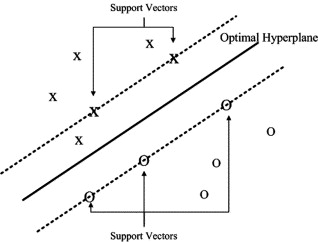
\includegraphics[height=4.34cm, width=6cm]{SVM}
		\caption{An overview  of an SVM \cite{Li2006772}}
		\label{fig:svm-overview}
	\end{figure}
	
	\subsubsection{Artificial Neural Network}
	An artificial neural network (ANN) is based on the functionality of the human brain \cite{Wang2003}. Neurons in the brain are interconnected and process information in parallel \cite{Wang2003}. A typical ANN is comprised of an input layer, $k$ number of hidden layers and an output layer. The neurons in each layer are connected to the neurons in the next layer. A numeric weight is defined between each pair of connected neurons. An activation function defines if a neuron will fire \cite{Wang2003}. The activation function bounds the value of a neuron to a specific range to limit the effect of divergent neurons \cite{Wang2003}. By using an activation function, a non-linear combination of weights can be generated \cite{Wang2003}. It has been proven that an ANN is able to approximate any continuous function if has at least one hidden node and an activation function that is both bounded to some range and non-constant \cite{Hornik1991251}.
	
	Extreme learning machines (ELM) is an alternative approach to the conventional back-propagated ANN. Huang \textit{el al.} \cite{Huang2006489} proved that the input and hidden layer weights can be randomly assigned if the activation function in the hidden layer is infinitely differentiable. By randomly assigning these weights, the weights for the output nodes can be determined analytically \cite{Huang2006489}. This allows ELMs to be trained orders of magnitude faster than a back-propagated ANN \cite{6035797, Huang2006489}. ELMs have been shown to provide better results than SVMs and ANNs on a variety of classification and regression tasks \cite{6035797, Huang2006489}.
	
	\subsubsection{Logistic Regression}
	Logistic regression is a technique that models the chance of an outcome based on the input features \cite{doi:10.11613/BM.2014.003}. Since chance is a ratio, the logarithm of the chance is modelled instead \cite{doi:10.11613/BM.2014.003}:
	log$(\frac{p}{1 - p}) = \beta_0 + \beta_1 x_1 + ... + \beta_m x_m$. $p$ represents the probability of an event (likelihood to default for example). $\beta_0$ represents the value of the criterion when the predictor is equal to 0. $\beta_1, ..., \beta_m$ are the regression coefficients associated with the $x_1, ..., x_m$ input features. The probability of an event can then be calculated as $p$ = $\frac{1}{1 + e^{-(\beta_0 + \beta_1 x_1 + ... + \beta_m x_m)}}$. A detailed overview of logistic regression can be found in \cite{Mood01022010} and \cite{doi:10.11613/BM.2014.003}.
	
	\subsubsection{$k$-Nearest Neighbours}
	The $k$-Nearest Neighbours ($k$NN) algorithm determines the output classification by examining the $k$ nearest training examples in the feature space \cite{6313426}. An input is classified by the majority vote of its neighbours.
	
	\subsubsection{Ensembles}
	An ensemble classifier is one which typically makes use of the aggregation of multiple classifiers. A single decision tree can be used for classification by branching on conjunctions of features and having the leaves represent the output class. A decision tree allows for easy interpretation of the generated model, however, typically provides relatively poor classification accuracy \cite{doi:10.1021/ci034160g}. 
	
	Random forest is a technique that fits a number of decision trees on random samples with replacement of the dataset. For each tree, $n$ features are randomly selected and the tree is grown \cite{WIDM:WIDM1072}. Samples that were not selected for training the tree is called out-of-bag data \cite{WIDM:WIDM1072}. It is used to test the error rate of the forest \cite{WIDM:WIDM1072, doi:10.1021/ci034160g}. The output classification is decided by the majority vote of each tree \cite{WIDM:WIDM1072}.
	
	Freund and Schapire's \cite{FREUND1997119} AdaBoost uses a weighted sum of multiple classifiers in order to determine the output. A classifier is constructed in an iterative fashion. At each iteration a pool of classifiers are considered and one classifier is added to the committee of classifiers. Input which is still misclassified is assigned a higher weight at each iteration \cite{Bergstra2006, rojas2009adaboost}. The aim is that the process will select a classifier which helps the still misclassified inputs. The chosen classifier is assigned a weight which determines its power in the overall classification \cite{Bergstra2006, rojas2009adaboost}. The sign of the function: $C(x) = \sum_{i=1}^{m} \alpha_i k_i$ is used to determine the final classification with $\alpha_i$ denoting the weight of each classifier $k_i$ \cite{Bergstra2006}. 
	
	\subsubsection{Naive Bayes}
	Naive Bayes makes an assumption that each input feature is independent of each other \cite{Lewis1998, rish2001empirical}. This allows multiple features be uncoupled from one another which simplifies the algorithm. Naive Bayes uses conditional probability to classify new inputs \cite{Lewis1998}. Using Bayes theorem, the following equation is derived: $p(C_i|\textbf{x}) = \frac{p(C_i) \times p(x_1|C_i) \times...\times p(x_n|C_i)}{p(\textbf{x})}$ with input $\textbf{x} = (x_1,...,x_n)$ and class label $C_i$ \cite{Lewis1998, rish2001empirical}. Since $p(\textit{x})$ is identical for each class, it is typically ignored \cite{rish2001empirical}. To classify an input, the probabilities for each class are calculated using the aforementioned equation and the output is the class with the highest probability \cite{Lewis1998}.
	
	The event model of Naive Bayes classification describes the assumed distribution of features. The Gaussian event model assumes that $p(x_i|C_i)$ follows a Gaussian distribution \cite{John:1995:ECD:2074158.2074196}. This allows support of continuous $x_i$ values \cite{John:1995:ECD:2074158.2074196}. The multivariate Bernoulli event model assumes that features are independent boolean values \cite{mccallum1998comparison}.
	
	\subsubsection{Clustering-launched classification}
	Clustering-launched classification (CLC) is a binary classifier. CLC first clusters the data into groups using a diverse hierarchical k-means algorithm \cite{Luo20097562}. The clusters are divided into positive subsets and negative subsets \cite{Luo20097562}. Support vectors are then used to separate the positive and negative subsets for each cluster \cite{Luo20097562}. Redundant or repeated support vectors are removed thereafter \cite{Luo20097562}.
	
	\subsection{Data Balancing algorithms}
	This section examines the different data balancing approaches and their respective algorithms.
	\subsubsection{Over-sampling}
	Random over-sampling (ROS) is a technique that randomly replicates examples in the minority class \cite{Batista:2004:SBS:1007730.1007735}. However, this technique can increase the likelihood of over-fitting since exact copies are made from the minority class \cite{Batista:2004:SBS:1007730.1007735}.
	
	The Synthetic minority over-sampling technique (SMOTE) \cite{Chawla:2002:SSM:1622407.1622416} forms new minority samples by interpolating along the line segment on some or all of the $k$ nearest minority class neighbours of a minority example. This approach attempts to alleviate the over-fitting that can occur from using random over-sampling.
	
	Adaptive synthetic sampling (ADASYN) \cite{4633969} is a variation of SMOTE which uses a weighed distribution for different minority class examples according to their difficulty in learning. More synthetic data is generated for minority class examples that are more difficult to learn compared to those that are easier to learn.
	
	\subsubsection{Under-sampling}
	Random under-sampling (RUS) is a technique that randomly eliminates examples in the majority class \cite{Batista:2004:SBS:1007730.1007735}. However, this technique can remove potentially useful information from the training set \cite{Batista:2004:SBS:1007730.1007735}. 
	
	Condensed Nearest Neighbour (CNN) rule \cite{1056066} finds a consistent subset of examples. A subset $D$ of $E$ is consistent if a 1-nearest neighbour classifier trained with $D$ correctly classifies $E$ \cite{Batista:2004:SBS:1007730.1007735}. The process draws one random majority class example and all minority class examples and puts them in $D$ \cite{Batista:2004:SBS:1007730.1007735}. Every misclassified example is then added from $E$ to $D$ \cite{Batista:2004:SBS:1007730.1007735}. This process attempts to remove examples that are far away from the decision border and therefore seen as less relevant for learning \cite{Batista:2004:SBS:1007730.1007735}.
	
	The Tomek link (TL) algorithm \cite{4309452} examines two examples $\textbf{x}_i$ and $\textbf{x}_j$ belonging to different classes. A TL occurs if there is not an example $\textbf{x}_k$ such that $d(\textbf{x}_i, \textbf{x}_k) < d(\textbf{x}_i, \textbf{x}_j)$ or $d(\textbf{x}_j, \textbf{x}_k) < d(\textbf{x}_j, \textbf{x}_i)$. If two examples form a TL then either one is noise or it is a borderline case \cite{Batista:2004:SBS:1007730.1007735}. This information can then be used to under-sample the majority class \cite{Batista:2004:SBS:1007730.1007735}.
	
	One-sided selection (OSS) \cite{Kubat97addressingthe} applies TL to remove borderline and noisy majority class examples then applies CNN to remove majority examples far from the decision border.
	
	Neighbourhood cleaning rule (NCL) \cite{Laurikkala:2001:IID:648155.757340} uses the edited nearest neighbour rule (ENN) to remove majority class examples. ENN removes examples whose label differs from the class of at least two of its nearest 3 neighbours. NCL examines each example $\textbf{x}_i$ and its 3 nearest neighbours. If $\textbf{x}_i$ belongs to the majority class and the neighbours contradict this class then $\textbf{x}_i$ is removed \cite{Batista:2004:SBS:1007730.1007735}. If $\textbf{x}_i$ belongs to the minority class and the neighbours contradict this class then the neighbours from the majority class are removed \cite{Batista:2004:SBS:1007730.1007735}.
	
	Instance threshold hardening (ITH) \cite{Smith:2014:ILA:2843614.2843686} uses the probability estimates from a classifier (such as SVM with a linear kernel) when k-fold cross validation is applied. It selects the $m$ examples from the majority class that have the highest probability estimates for that class when tested in k-fold cross validation. $m$ is the number of samples in the minority class.
	
	NearMiss-1 (NM-1) \cite{mani2003knn} picks majority class examples which have the smallest average distance to the three nearest minority class examples.
	
	Cluster centroids (CC) applies the $k$-means algorithm with $m$ clusters to the majority class and uses the coordinates of the cluster centroids as the majority samples. As in ITH, $m$ is the number of samples in the minority class.	
	
	\subsubsection{Combination}
	SMOTE + TL \cite{batista2003balancing} first applies SMOTE then applies TL. Applying SMOTE can cause minority samples to extend too deep into the majority class space or the opposite where majority class samples extend too deep into the minority class space \cite{batista2003balancing}. TL is used as a data cleaning method to remove examples from both classes to produce well-defined class clusters \cite{batista2003balancing}.
	
	SMOTE + ENN works similarly to SMOTE + TL but ENN is more aggressive at removing samples than TL \cite{Batista:2004:SBS:1007730.1007735}.
	
	\subsection{Evaluation metrics}
	The number of true positives (TP), true negatives (TN), false positives (FP) and false negatives (FN) are used to define several metrics which are used to compare the results in this paper. The true positive rate (TPR) or sensitivity defines the proportion of actual positives which are predicted as positive. The TPR is calculated as $\frac{TP}{TP + FN}$. The true negative rate (TNR) or specificity defines the proportion of actual negatives which are predicted as negative. The TNR is calculated as $\frac{TN}{TN + FP}$. 
	
	Accuracy is typically a poor measure of quality for imbalanced datasets as classifiers tend to bias towards the majority class \cite{Batista:2004:SBS:1007730.1007735, Chawla:2004:ESI:1007730.1007733}. Several balanced performance metrics are used instead. The balanced accuracy (BACC) provides an equal weighting in TPR and TNR. It is calculated as $\frac{TPR + TNR}{2}$. Matthews correlation coefficient (MCC) also provides a balanced measure of classification quality and is scored between -1 and 1. The MCC is calculated as: $\frac{(TP \times TN) - (FP \times FN)}{\sqrt{(TP + FP)(TP + FN)(TN + FP)(TN + FN)}}$.
	
	
	\section{Experimental design and evaluation}
	A systematic experimental design was developed to ensure repeatable results.
	\subsection{Experimental Approach}
	\label{method-approach}
	
	We aim to evaluate a set of statistical and machine learning classification techniques on treatment default data sets and compare it to that applied to other related classification datasets. A variety of classification techniques were chosen to test against: ANN, SVM using a linear, RBF and polynomial kernel, logistic regression, decision tree, AdaBoost, random forest, $k$NN, Gaussian naive Bayes, Bernoulli naive Bayes, ELM and CLC. These were chosen to include a selection of well known techniques, ensemble techniques and newer techniques that have shown promising results in other studies. 
	
	There are typically substantially fewer defaulters than those cured. However, most classification algorithms expect a 50:50 split between classes. We therefore include an analysis of several data balancing algorithms: CC, ENN, IHS, NM-1, NCR, OSS, RUS, TL, ADASYN, ROS, SMOTE, ensemble of SMOTE + EEN and ensemble of SMOTE + TL. These balancing techniques were chosen to facilitate an evaluation of both over-sampling and under-sampling techniques. Included in the evaluation is techniques that use simple approaches and as others that use sophisticated algorithms.
	
	All the experiments use stratified 5-fold validation to divide a single dataset into multiple training and testing datasets. Stratified $k$-fold divides the dataset into $k$ segments and ensures that each segment contains the same ratio of positive and negative examples as the dataset as a whole. $k$ training and testing sets are created by using one segment as the testing dataset and every other segments as the training data. This is repeated such that every segment is used as testing data. Results for each fold are then averaged before being presented. 5-fold was used instead of 10-fold to ensure that there was a reasonable sample of defaulters per fold.
	
	All data is first pre-processed before it is used for each experiment. The median, mean or most frequent value are common approaches to fill in  missing values for examples. Another approach is to remove examples that contain missing values. We opted to remove examples with missing data to prevent it  causing bias in our classification. Most classification techniques are not equipped to handle categorical data. To address this issue, we use ``one-hot encoding" to encode a feature with $n$ categories into $n$ separate binary features corresponding to each category. The feature that corresponds with the categorical value is set to 1 while the other $n-1$ features are set to 0. We standardise all numeric features to ensure that it has zero mean and unit variance since most classifiers expect features to have a normal distribution. For each fold, the mean and standard deviation are derived from the training set and then used to standardise both the training and testing set. 
	
	\subsubsection{Parameter tuning}
	\label{parameter_tuning}
	As part of the evaluation of the different classification  parameter tuning is for our datasets and its effect on each classifier. We also want to see if just the addition of a data balancing algorithm can improve the classification. We first test each classifier at its default parameters. In the case where a classifier does not have default parameters available, we provide our own reasonable defaults and label those classifiers accordingly. To see the effect of a data balancing algorithm on the classifiers with default parameters, we will use the data balancer that results in the highest BARR. Finally, for each classifier we search a grid of reasonable parameters and select the parameters that yield the highest BARR. The grid includes the parameters of the classifier as well as the different data balancing techniques.
	
	Over-fitting the classifiers is a concern when applying the grid search. To prevent the classifiers from over-fitting the parameter grid is kept fairly coarse and three runs of stratified 5-fold cross-validation is executed and the results averaged. To provide fair comparison between parameter sets and to facilitate repeatability, the data balancer, stratified $k$-fold algorithm and classifier itself use fixed initialisation values. These initialisation values differ across each of the three runs. This ensures that each parameter set utilises the same training and testing folds per run but that these folds differ across runs. The initialisation values are saved in the experiment results to facilitate reproducibility. We chose BARR to compare the results between classifiers and scenarios.	
	
	\subsubsection{Comparison of classification techniques}
	\label{comparision_of_classification_technique}
	This experiment focuses on comparing each optimised classifier in detail. The same testing procedure is used as outlined in section \ref{parameter_tuning} except in this experiment we record several additional metrics to compare the classification techniques in detail: TPR, TNR, BARR, MCC, informedness and time to fit each training fold. In addition, a receiver operating characteristic (ROC) curve is also plotted as an additional means of comparing the classification techniques and to indicate what TPR can be achieved for an acceptable false positive rate (FPR). To determine how the results generalise against the other classification datasets, a final scatter plot is presented which compares difference of TPR and FPR from the median of each for every classifier on every dataset.
	
	The recorded metrics will allow us to determine which classifier is best suited for our treatment default datasets but also allow us to see if the results generalise to the credit default datasets and to reason over why we see those results.
	
	\subsubsection{Comparison of data balancing algorithms}
	We would like to investigate each data balancing technique against each classifier. We use our parameter grid results from section \ref{parameter_tuning} to obtain the optimal parameters for each classifier on every data balancing algorithm. As before, the highest BARR is used to determine these optimal parameters. To ensure repeatable results, 10 runs of stratified 5-fold cross validation is executed and the results averaged. A set of unique randomly selected initialisation keys used for each run and recorded with the results. These are used so that $k$-fold cross validation, data balancing and classification algorithms produce deterministic output.
	
	A bar chart is plotted with each classifier against the BARR for the treatment default datasets. As in section \ref{comparision_of_classification_technique}, a scatter plot is presented which compares difference of true positive and false positive from the median of each for each classifier on each data balancing algorithm on each dataset. 
	
	\subsubsection{Comparison of feature selection algorithms}
	Feature selection can be used to help remove noisy features that do not contribute to the overall classification \cite{Guyon:2003:IVF:944919.944968}. It can also speed up training times for large datasets \cite{Guyon:2003:IVF:944919.944968}. Aside from the aforementioned benefits, we want to use feature selection to get a better understanding of how the features are being utilised by each classifier. Typically only classifiers that create a model with some linear combination of features can be easily interpreted.
	
	A number of feature selection strategies were selected for this experiment: Analysis of variance (ANOVA) F-value with $\chi^2$ tests, logistic regression, linear SVM, Bernoulli naive Bayes, decision tree, random forest. The feature selection is calculated on the training examples and not the entire dataset to prevent bias in our results \cite{PMID:25988841}.
	
	The ANOVA F-test is used on numeric features and $\chi^2$ test on categorical features. The ANOVA F-test tests the null hypothesis that 2 or more groups have the same population mean. The $\chi^2$ test the null hypothesis that features that are independent of its class and therefore not relevant to the classification. We chose a p-value of 0.1 to reject each of the null hypotheses. 
	
	We measure our other feature selection techniques in two different ways. In the first approach we use the median feature weight as the threshold and only keep features that are rated more important. We want to identify the technique that can retain the most important features for our different classifiers and will therefore result in the lowest reduction in BARR. In the second approach we apply recursive feature elimination (RFE) in order to identify the optimal number of parameters for the particular technique. RFE removes the least important feature at each iteration until only one feature remains. Good feature selection techniques should be able to reduce the overall features while retaining or even improving the classification. For each feature selection technique the set of features that result in the highest BARR are retained. For some training folds, this could result in no features being removed. 
	
	To test the feature selection strategies we record the BARR of each classifier with each feature selection strategy. For the RFE approach the minimum features, maximum features and average features selected is also recorded since each fold of the $k$-fold cross-validation could have a different number of features selected.
	
	\subsubsection{An analysis of time to default in the Lima Peru dataset}
	We want to determine if the time it takes for an individual to default affects their classification ``profile''. We use several default ranges: 0-30 days, 0-60 days, 0-100 days, 0-200 days, 50-100 days, 100-200 days, 200-1000 days, 300-1000 days. The non-defaulters are randomly divided into to two sets. The first set is joined with the defaulters in the range and used as the training set while the other set is joined with the defaulters outside the range and used as the testing set. This process is repeated over 100 runs and the results are then averaged. A set of unique random initialisation keys are generated for each run. This is used to ensure that the split of non-defaulters is the same for each default range and that each data balancer and classifier gets the same initialisation values. If the time to default does not play a large role in the classification then we except to see similar results for each default range. If it does play a large role then we expect to see poor classification results and variability in results between default ranges.
	
	
	\subsection{Datasets}
	The experiments were run on a set of real-world datasets: one TB default dataset from Lima Peru \cite{Lackey:10356751520150601} and two credit scoring datasets. The TB dataset was obtained from the Dryad digital repository. The two credit scoring datasets (later referred to as the German and Australian dataset) were obtained from the UCI machine learning repository \cite{Lichman:2013}. Table \ref{table:data_sets} provides an overview of the characteristics of the datasets. The Peru TB dataset is highly imbalanced which makes it an ideal dataset to test different balancing algorithms. The German dataset is slightly imbalanced while the Australian dataset is balanced. The Peru data set came with values pre-discretized and therefore only contains categorical features.
	\begin{table*}
		\centering
		\caption{Data set summary}
		\label{table:data_sets}
		\makebox[\linewidth]{
		\begin{tabular}{c|c|c|c|c} \hline	
			Data set&Entries&Number of numerical features&Number of categorical features&Data balance ratio (Cured:Default)\\ \hline
			Lima Peru TB \cite{Lackey:10356751520150601}&1186&0&15&8.65:1 \\
			German Credit Scoring&1000&7&13&2.33:1 \\
			Australian Credit Scoring&690&6&8&1.25:1
		\end{tabular}
		}
	\end{table*}

	\subsection{Limitations}
	While our approach has been designed to limit bias and over-fitting as far as possible, the scale of our comparison and size of our datasets could introduce over-fitting nonetheless. For this reason, our observations and conclusions incorporate the use of trends, prior knowledge and comparison to our other datasets. 
	
	\section{Software development}
	This section outlines the software development methodology and details of the implementation.
	\subsection{Development principles and methodology}
	Throughout this project we strived to ensure that our software is highly configurable and modular such that core components can be re-used for each experiment. Our goal was to create a system that could support multiple datasets and classifiers in a generic manner. We wanted the system to handle the entire experimental process including pre-processing and result visualisation.
	
	We followed an iterative development methodology in our software. We used feedback from our weekly meeting to improve our experimental methodology and visualisation of results.
	
	\subsection{Implementation details}
	We developed the system in Python 2.7 since it has widespread library support and facilitates quick development. We support datasets formatted as a comma separated values (CSV) file and allow new binary classification datasets to be supported with the addition of just ten lines in the configuration file. All pre-processing operations such as removal of examples with missing values, creation of dummy variables and scaling of data are executed within the code base.
	
	To support a wide variety of techniques, we used several pre-existing libraries for our classification and data balancing techniques. We used scikit-learn \cite{scikit-learn} for most of the classification techniques with the exception of ELM and CLC. Akusok \textit{et al.}'s \cite{7140733} Python ELM toolbox was used for the implementation of the ELM. The CLC implementation was obtained from the original authors \cite{Chen2006} as a compiled C++ executable. By creating a wrapper, we can support classifiers written in different languages or which have a different interface. We used wrappers to provide a scikit-learn interface for the ELM and CLC classifier. In addition, the CLC classifier expects a tab separated values (TSV) file as input and produces the classification model and predictions as a TSV file. The wrapper is used to accommodate this.
	
	Different data balancing techniques can be used per classifier. For the data balancing algorithms, we used Lema\^{i}tre \textit{et al.}'s \cite{lemaitre2016imbalanced} imbalanced-learn package to provide a scikit-learn compatible implementation.
	
	Every dataset can use its own configuration file which contains the parameters to use for each classifier as well as which data balancing algorithm to use alongside each classifier. Classifiers and datasets can be easily enabled or disabled as desired. We have already provided a reasonable search space in our parameter tuning algorithm. However, it is simple to modify or add a new parameter tuning configuration file if a more fine-grained search is required.
	
	After each experiment is completed, the statistics of it will be computed and saved as a CSV file. The relevant graphs will also be generated and saved. These have been used in section \ref{results}.
	
	The system has been designed that it can execute the aforementioned experiments for any binary classification problem not just the ones outlined in this paper. With some modifications, it could also be extended to support multi-class classification problems too. The code has been written in a generic manner that reduces the need to replicate code. This allows new experiments to be created with minimal overhead. Each experiment is also multi-threaded to reduce the execution time.
	
	\section{Results and discussion}
	This section presents and discusses the results of the experiments outlined in section \ref{method-approach}.
	\subsection{Parameter Tuning}
	
	
	\begin{figure*}
		\centering
		\makebox[\linewidth]{
		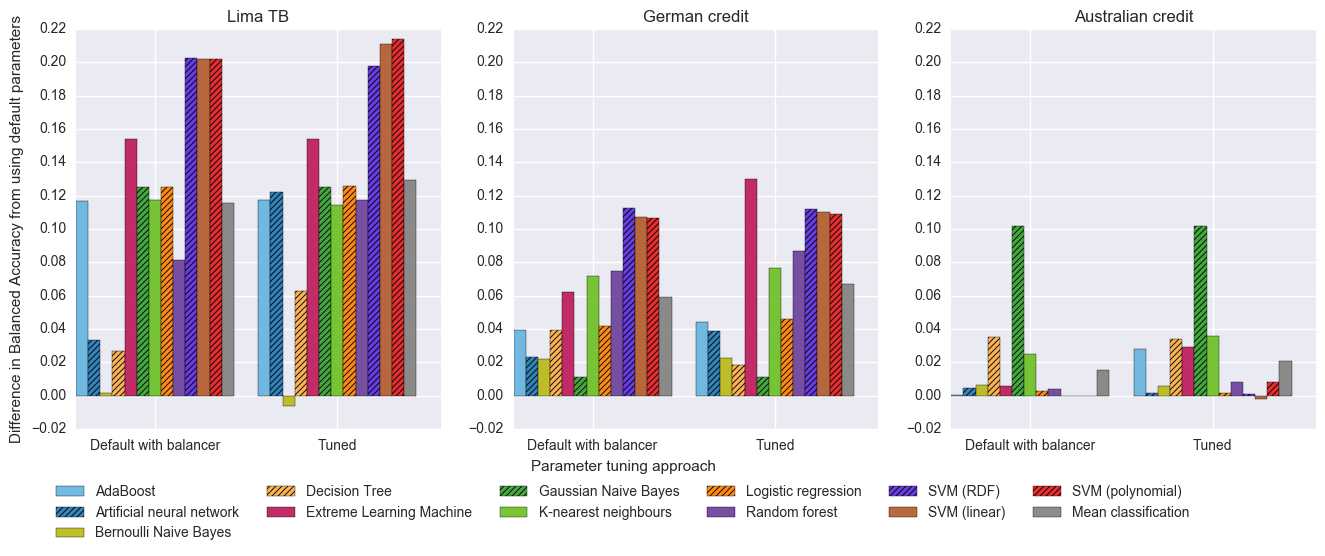
\includegraphics[scale=0.55]{Parameter_tuning_approach_results_per_classifier_plot_['Lima_TB',_'German_credit',_'Australian_credit']_Balanced_Accuracy_2016-10-24_21-47-19}}
		\caption{Difference in balanced accuracy from using default parameters with different parameter tuning approaches}
		\label{fig:res}
	\end{figure*}

	\begin{figure*}
		\centering
		\makebox[\linewidth]{
			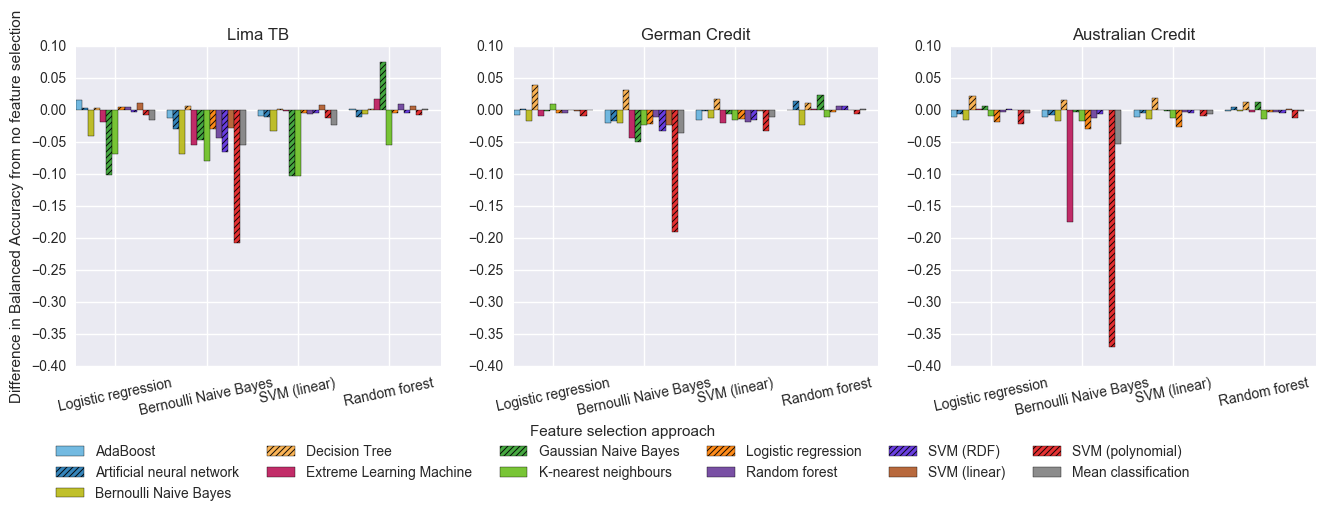
\includegraphics[scale=0.62]{Feature_selection_approach_results_per_classifier_plot_['Lima_TB',_'German_Credit',_'Australian_Credit']_Balanced_Accuracy_2016-10-26_15-56-32}}
		\caption{Difference in balanced accuracy from using no feature selection with different feature selection approachs for each classifier}
		\label{fig:res}
	\end{figure*}

	\begin{figure*}
		\centering
		\vspace*{-1.5cm}\hspace*{-1.5cm}\begin{subfigure}{.5\textwidth}
			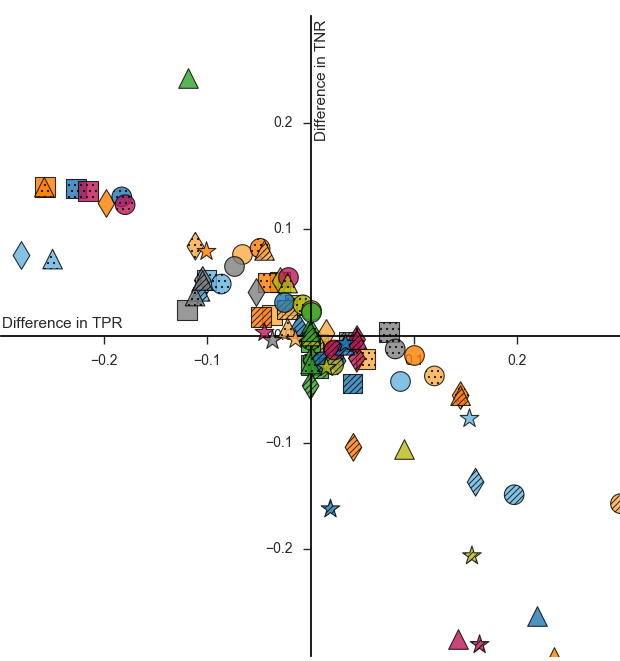
\includegraphics[scale=0.61]{classifier_dataset_plt_2016-10-26_18-44-26}
			\label{fig:res}
		\end{subfigure}\hspace*{4cm}\vspace*{-0.5cm}%
		\hspace*{-2cm}\begin{subfigure}{.5\textwidth}
			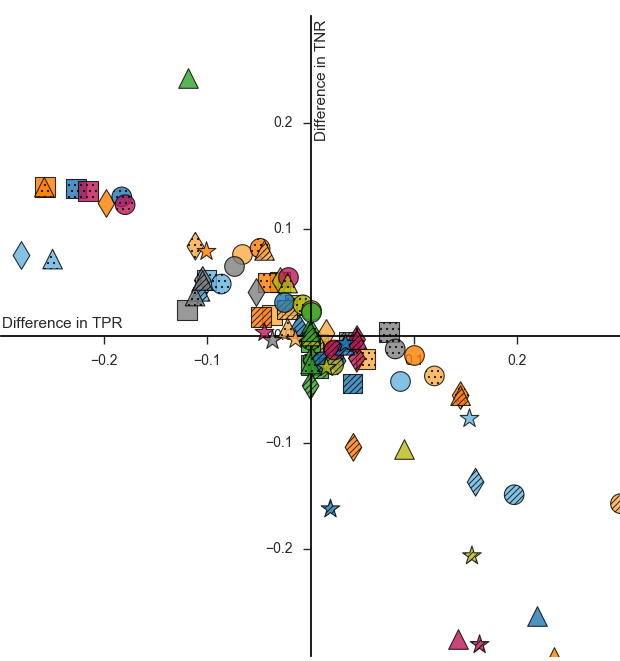
\includegraphics[scale=0.61]{classifier_dataset_plt_2016-10-26_18-44-26}
			\label{fig:res}
		\end{subfigure}
		\vspace*{-0.5cm}\hspace*{-3cm}\begin{subfigure}{\textwidth}
			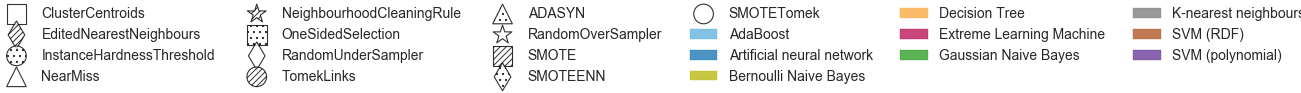
\includegraphics[scale=0.6]{legend}
			\label{fig:res}
		\end{subfigure}
		\caption{Comparison of classifiers with different data balancing techniques on Lima TB data set (left) and [PLACEHOLDER for DIMAGI attrition] (right). SVM and Logistic regression excluded because of minimal variation.}
	\end{figure*}
	

	\label{results}
	\begin{enumerate}
		\item Tables with true positive, true negative, false positive and false negative rate for each classifier on each dataset
		\item ROC curves which can be used to determine true positive for an acceptable amount of false positives for each classification technique on each dataset
		\item Graphs which outline difference in accuracy of each data balancing technique for each dataset
		\item Discussion on best classification technique
		\item Discussion on data balancing results
		\item Outline similarities and differences in results between the two TB datasets and between TB and financial datasets and determine if they are similar enough that results for the German and Australian credit scoring datasets could be used for the two TB datasets.
	\end{enumerate}
	
	\section{Conclusions and Future Work}
	\begin{enumerate}
		\item Likely something along the lines of utilising more temporal based data so that classification is not just done at registration but also at each check-up for example. Future work may also be the testing of more classification techniques as well as datasets from other parts of the world.
	\end{enumerate}
	
	%
	% The following two commands are all you need in the
	% initial runs of your .tex file to
	% produce the bibliography for the citations in your paper.
	\bibliographystyle{abbrv}
	\bibliography{sigproc}  % sigproc.bib is the name of the Bibliography in this case
	% You must have a proper ".bib" file
	%  and remember to run:
	% latex bibtex latex latex
	% to resolve all references
	%
	%\balancecolumns
\end{document}
